\documentclass{article}
\usepackage{amsmath}
\usepackage{amsfonts}
\usepackage[a4paper,width=140mm,top=15mm,bottom=15mm]{geometry}
\usepackage{hyperref}
\usepackage{mathtools}
\usepackage{graphicx}
\graphicspath{ {./figures/} }

\hypersetup{
    colorlinks,
    citecolor=black,
    filecolor=black,
    linkcolor=black,
    urlcolor=black
}

\DeclareUnicodeCharacter{2212}{-}




\title{Esercizi}
\author{Michele Leigheb}
\date{}
\begin{document}
\maketitle
\tableofcontents{}
\section{Complessi}
\begin{itemize}
	\item \(\displaystyle 2^{(a+ib)} = 2^a (\cos(b \ln(2)) + i\sin(b \ln(2))) \)
	\item \(\displaystyle 3^{(a+ib)} = 3^a (\cos(b \ln(3)) + i\sin(b \ln(3))) \)
	\item \(\displaystyle e^{(a+ib)} = e^a (\cos(b)) + i\sin(b) \)
	\item \(\displaystyle \alpha^{(a+ib)} = e^{\alpha} (\cos(b)\ln(\alpha)) + i\sin(b\ln(\alpha)) \)
\end{itemize}



\section{Esercizi}

\section{Esercizio 144 }
 Studiare il sistema \[S:\begin{cases}\overset{\cdot}{x} = \left(\begin{matrix}2 & 0 & 0\\-3 & 0 & 1\\3 & 1 & 0\end{matrix}\right) x+ \left(\begin{matrix}1\\-2\\2\end{matrix}\right)u\\y = \left(\begin{matrix}-2 & -1 & 1\end{matrix}\right) x +\left(\begin{matrix}0\end{matrix}\right) u\end{cases}\]
\subsection{Studio Osservabilità}

Studiamone l’osservabilità. Calcoliamo allora O e troviamo I = ker(O):
\[
 O = \begin{pmatrix}C \\ CA \\ CA^2 \end{pmatrix} = \left(\begin{matrix}-2 & -1 & 1\\2 & 1 & -1\\-2 & -1 & 1\end{matrix}\right), |O| = 0 \]

O ha rango $ 1 $ quindi il suo nucleo ha dimensione $ 2 $.

Calcolando trovo \[ 
I = ker(O) = \left[ \left(\begin{matrix}-1\\2\\0\end{matrix}\right), \  \left(\begin{matrix}1\\0\\2\end{matrix}\right)\right]\]

E $T^{-1}$ viene \[ 
T^{-1} = \left(\begin{matrix}-1 & 1 & 0\\2 & 0 & 0\\0 & 2 & 1\end{matrix}\right) \]
\[ 
T = \left(\begin{matrix}0 & \frac{1}{2} & 0\\1 & \frac{1}{2} & 0\\-2 & -1 & 1\end{matrix}\right) \]Calcoliamo allora le matrici del sistema, e vedremo che risultano partizionate come avevamo previsto:
\[ 
\overset{\sim}{A} = T A  T^{-1} = \left(\begin{matrix}0 & \frac{1}{2} & 0\\1 & \frac{1}{2} & 0\\-2 & -1 & 1\end{matrix}\right)\left(\begin{matrix}2 & 0 & 0\\-3 & 0 & 1\\3 & 1 & 0\end{matrix}\right)\left(\begin{matrix}-1 & 1 & 0\\2 & 0 & 0\\0 & 2 & 1\end{matrix}\right) = \left(\begin{matrix}\frac{3}{2} & - \frac{1}{2} & \frac{1}{2}\\- \frac{1}{2} & \frac{3}{2} & \frac{1}{2}\\0 & 0 & -1\end{matrix}\right) \]
\[ 
\overset{\sim}{C} = CT^{-1} = \left(\begin{matrix}-2 & -1 & 1\end{matrix}\right)\left(\begin{matrix}-1 & 1 & 0\\2 & 0 & 0\\0 & 2 & 1\end{matrix}\right) = \left(\begin{matrix}0 & 0 & 1\end{matrix}\right) = ( 0\ \ \overset{\sim}{C}_2) \]
Con le matrici \[ A_{11} = \left(\begin{matrix}\frac{3}{2} & - \frac{1}{2}\\- \frac{1}{2} & \frac{3}{2}\end{matrix}\right) , A_{22} = \left(\begin{matrix}-1\end{matrix}\right) \]Quindi infine mi viene che gli autovalori osservabili sono $ -1\  $ e gli inosservabili sono $ 2\ 1\  $.

\subsection{Studio Raggiungibilità}
Ora per studiare la raggiungibilità degli stati calcolo $R = (B\ AB\ ...\ A^{n-1}B)$: \[ R = \left(\begin{matrix}1 & 2 & 4\\-2 & -1 & -5\\2 & 1 & 5\end{matrix}\right), |R| = 0 \] 

Vediamo che $rango(R) = 2$ e quindi : \[ \mathfrak{R} = \left[ \left(\begin{matrix}1\\-2\\2\end{matrix}\right), \  \left(\begin{matrix}2\\-1\\1\end{matrix}\right)\right] \]

Tutti gli stati che hanno questa struttura sono, allora, raggiungibili. Mettiamo in evidenza questa struttura;
cambiamo base, e vorremmo avere lo stato espresso come $z = Tx$ tale che, se x è uno stato raggiungibile, allora: \[ z_R = T x_R = \begin{pmatrix} \star  \\ 0 \\0\end{pmatrix}\]

E $T^{-1}$ viene \[ T^{-1} = \left(\begin{matrix}1 & 2 & 0\\-2 & -1 & 0\\2 & 1 & 1\end{matrix}\right) \Longrightarrow T = \left(\begin{matrix}- \frac{1}{3} & - \frac{2}{3} & 0\\\frac{2}{3} & \frac{1}{3} & 0\\0 & 1 & 1\end{matrix}\right) \]
\[ \overset{\sim}{A} = T A  T^{-1} = \left(\begin{matrix}- \frac{1}{3} & - \frac{2}{3} & 0\\\frac{2}{3} & \frac{1}{3} & 0\\0 & 1 & 1\end{matrix}\right)\left(\begin{matrix}2 & 0 & 0\\-3 & 0 & 1\\3 & 1 & 0\end{matrix}\right)\left(\begin{matrix}1 & 2 & 0\\-2 & -1 & 0\\2 & 1 & 1\end{matrix}\right) = \left(\begin{matrix}0 & 2 & - \frac{2}{3}\\1 & 1 & \frac{1}{3}\\0 & 0 & 1\end{matrix}\right) \]Con le matrici \[ \overset{\sim}{A}_{11} = \left(\begin{matrix}0 & 2\\1 & 1\end{matrix}\right) , \overset{\sim}{A}_{22} = \left(\begin{matrix}1\end{matrix}\right)  \]e le matrici \[ \overset{\sim}{B} = TB = \left(\begin{matrix}1\\0\\0\end{matrix}\right)  \]
Ora ne calcoliamo la raggiungibilità: \[ \overset{\sim}{H}(t) = e^{\overset{\sim}{A}t}\overset{\sim}{B} = \begin{pmatrix} e^{\overset{\sim}{A}_{11}t} &  \star \\ 0 & e^{\overset{\sim}{A}_{22}t} \end{pmatrix} \begin{pmatrix} \overset{\sim}{B}_1 \\ 0 \end{pmatrix} = \begin{pmatrix} e^{\overset{\sim}{A_{11}t}}\overset{\sim}{B_1} \\ 0 \end{pmatrix} \]
Quindi infine mi viene che gli autovalori ragg sono $ 2, -1,  $ e gli irrag sono $ 1,  $
\subsection{Scomposizione di Kalman}
I miei sottospazi di riferimento sono:	\[ \mathfrak{I} = \left[ \left(\begin{matrix}-1\\2\\0\end{matrix}\right), \  \left(\begin{matrix}1\\0\\2\end{matrix}\right)\right], \mathfrak{R} = \left[ \left(\begin{matrix}1\\-2\\2\end{matrix}\right), \  \left(\begin{matrix}2\\-1\\1\end{matrix}\right)\right] \]
La matrice dei vettori di base di I e R è \[ \chi_1 =  \left(\begin{matrix}1\\-1\\1\end{matrix}\right) \]
Ci sono più righe che colonne quindi sicuro l'intersezione c'è.

\paragraph{Per quanto riguarda Chi2:} $ \chi_2 | \chi_2 \oplus \chi_1 = \mathfrak{R} $ è \[ \chi_2 = \left(\begin{matrix}1\\-2\\2\end{matrix}\right) \]

\paragraph{Per quanto riguarda Chi3:} $ \chi_3 | \chi_3 \oplus \chi_1 = \mathfrak{I} $ è \[ \chi_3 = \left(\begin{matrix}-1\\2\\0\end{matrix}\right) \]

\paragraph{Per quanto riguarda Chi4:} $ \chi_4 | \chi_1 \oplus \chi_2 \oplus  \chi_3 \oplus \chi_4 = \mathbb{R} $ è \[ \chi_4 = \left(\begin{matrix}\end{matrix}\right) \]
\paragraph{Ora facciamo T inversa:} \[ T^{-1} = (\chi_1\ \chi_2\ \chi_3\ \chi_4\ ) = \left(\begin{matrix}1 & 1 & -1\\-1 & -2 & 2\\1 & 2 & 0\end{matrix}\right) \]
e quindi \[T = \left(\begin{matrix}2 & 1 & 0\\-1 & - \frac{1}{2} & \frac{1}{2}\\0 & \frac{1}{2} & \frac{1}{2}\end{matrix}\right)\]
\[ \widetilde{A} = TAT^{-1} = \left(\begin{matrix}1 & 0 & 1\\1 & \frac{1}{2} & - \frac{1}{2}\\0 & \frac{1}{2} & \frac{1}{2}\end{matrix}\right) * T^{-1} = T*\left(\begin{matrix}2 & 2 & -2\\-2 & -1 & 3\\2 & 1 & -1\end{matrix}\right) =\left(\begin{matrix}2 & 3 & -1\\0 & -1 & 0\\0 & 0 & 1\end{matrix}\right) \]

\[ \widetilde{B} = T B = \left(\begin{matrix}0\\1\\0\end{matrix}\right) \]

\[ \widetilde{C} = C T^{-1} = \left(\begin{matrix}0 & 2 & 0\end{matrix}\right) \]
\[Phi(t) = \left(\begin{matrix}e^{2 t} & e^{2 t} - e^{- t} & - e^{2 t} + e^{t}\\0 & e^{- t} & 0\\0 & 0 & e^{t}\end{matrix}\right) \]

\subsection{Studio Funzione di trasferimento}

\[ (sI-A) = \left(\begin{matrix}s - 2 & 0 & 0\\3 & s & -1\\-3 & -1 & s\end{matrix}\right), |sI-A| = \left(s - 2\right) \left(s - 1\right) \left(s + 1\right) \]
\[ \Phi(s) = (sI-A)^{-1} = \frac{\left(\begin{matrix}s^{2} - 1 & 0 & 0\\3 - 3 s & s \left(s - 2\right) & s - 2\\3 s - 3 & s - 2 & s \left(s - 2\right)\end{matrix}\right)}{\left(s - 2\right) \left(s - 1\right) \left(s + 1\right)} \]

Le funzioni caratteristiche sono \[\begin{array}{rcl}  H(s) & = & \Phi(s)B \\ \Psi(s) & = & C \Phi(s)\\ W(s) & = & C(sI-A)^{-1}B  \end{array} \]

e quindi \[ H(s)  =  \frac{\left(\begin{matrix}s^{2} - 1\\- 2 s^{2} + 3 s - 1\\2 s \left(s - 2\right) + s + 1\end{matrix}\right)}{\left(s - 2\right) \left(s - 1\right) \left(s + 1\right)} \ \Psi(s) = \frac{\left(\begin{matrix}- 2 s^{2} + 6 s - 4 & - s \left(s - 2\right) + s - 2 & s \left(s - 2\right) - s + 2\end{matrix}\right)}{\left(s - 2\right) \left(s - 1\right) \left(s + 1\right)} \]
\[ W(s)  =  \frac{\left(\begin{matrix}2 s \left(s - 2\right) - 2 s + 4\end{matrix}\right)}{\left(s - 2\right) \left(s - 1\right) \left(s + 1\right)}   \] 
Il grafico di bode è:
\[ W(s) = \frac{2 \left(s - 2\right) \left(s - 1\right)}{\left(s - 2\right) \left(s - 1\right) \left(s + 1\right)} \]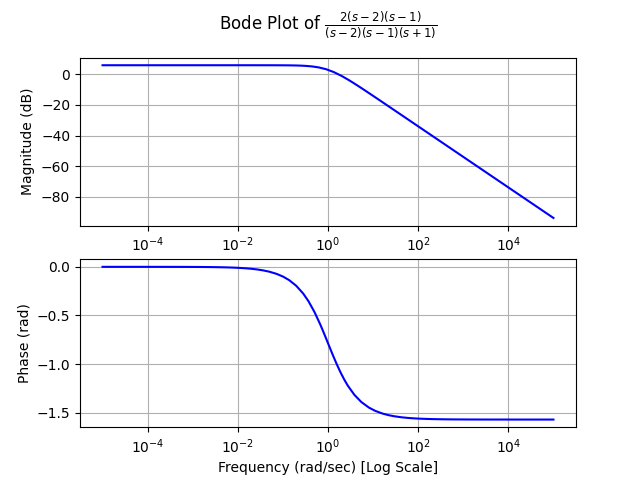
\includegraphics[scale = 0.5]{figures/bode_5908268.png}


Il grafico di Nyquist è:
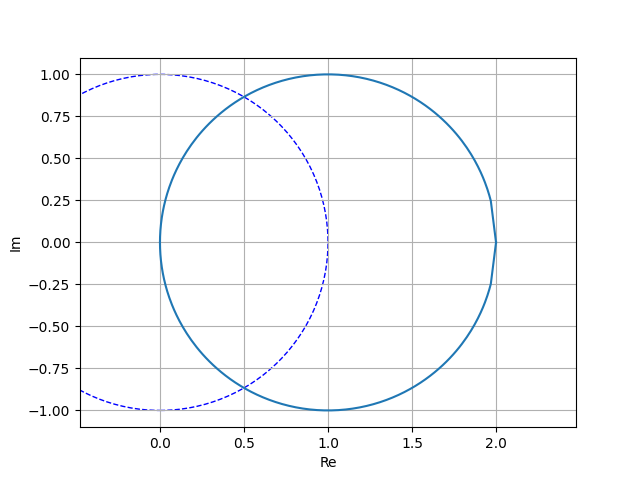
\includegraphics[scale = 0.5]{figures/nyquist_5514408.png}nel tempo continuo è \[ 2 e^{- t} \theta\left(t\right) \]
\subsubsection{Vediamo le risposte:}
\[ u(t) = 2 t \theta\left(t\right) \to U(s) = \mathcal{L}[u(t)] = \frac{2}{s^{2}} \]
\[ y_F(s) = W(s) U(s)  = \left(\begin{matrix}\frac{4}{s^{2} \left(s + 1\right)}\end{matrix}\right)\] 

\[ y_F(t) = \mathcal{L}^{-1}[y_F(s)] = \left(\begin{matrix}4 \left(\left(t - 1\right) e^{t} + 1\right) e^{- t} \theta\left(t\right)\end{matrix}\right) \]
\[ u(t) = 2 t \theta\left(t - 1\right) \to U(s) = \mathcal{L}[u(t)] = \frac{2 \left(s + 1\right) e^{- s}}{s^{2}} \]
\[ y_F(s) = W(s) U(s)  = \left(\begin{matrix}\frac{4 e^{- s}}{s^{2}}\end{matrix}\right)\] 

\[ y_F(t) = \mathcal{L}^{-1}[y_F(s)] = \left(\begin{matrix}- 4 \left(\log{\left(e^{- t} \right)} + 1\right) \theta\left(t - 1\right)\end{matrix}\right) \]
\[ u(t) = - \theta\left(t\right) \to U(s) = \mathcal{L}[u(t)] = - \frac{1}{s} \]
\[ y_F(s) = W(s) U(s)  = \left(\begin{matrix}- \frac{2}{s \left(s + 1\right)}\end{matrix}\right)\] 

\[ y_F(t) = \mathcal{L}^{-1}[y_F(s)] = \left(\begin{matrix}2 \cdot \left(1 - e^{t}\right) e^{- t} \theta\left(t\right)\end{matrix}\right) \]
\[ u(t) = - \theta\left(t - 1\right) \to U(s) = \mathcal{L}[u(t)] = - \frac{e^{- s}}{s} \]
\[ y_F(s) = W(s) U(s)  = \left(\begin{matrix}- \frac{2 e^{- s}}{s \left(s + 1\right)}\end{matrix}\right)\] 

\[ y_F(t) = \mathcal{L}^{-1}[y_F(s)] = \left(\begin{matrix}2 \left(e - e^{t}\right) e^{- t} \theta\left(t - 1\right)\end{matrix}\right) \]
\[ u(t) = \cos{\left(t \right)} \theta\left(t\right) \to U(s) = \mathcal{L}[u(t)] = \frac{s}{s^{2} + 1} \]
\[ y_F(s) = W(s) U(s)  = \left(\begin{matrix}\frac{2 s}{s^{3} + s^{2} + s + 1}\end{matrix}\right)\] 

\[ y_F(t) = \mathcal{L}^{-1}[y_F(s)] = \left(\begin{matrix}\left(\sqrt{2} e^{t} \sin{\left(t + \frac{\pi}{4} \right)} - 1\right) e^{- t} \theta\left(t\right)\end{matrix}\right) \]
\[ u(t) = \cos{\left(t \right)} \theta\left(t - 1\right) \to U(s) = \mathcal{L}[u(t)] = \frac{\left(\left(s - i\right) e^{s - i} + \left(s + i\right) e^{s + i}\right) e^{- 2 s}}{2 \left(s - i\right) \left(s + i\right)} \]
\[ y_F(s) = W(s) U(s)  = \left(\begin{matrix}\frac{\left(s + s e^{2 i} - i + i e^{2 i}\right) e^{- s - i}}{s^{3} + s^{2} + s + 1}\end{matrix}\right)\] 

\[ y_F(t) = \mathcal{L}^{-1}[y_F(s)] = \left(\begin{matrix}\frac{\left(1 - i\right) \left(1 + i\right) \left(e^{t - 1} \sin{\left(t \right)} + e^{t - 1} \cos{\left(t \right)} - \sin{\left(1 \right)} - \cos{\left(1 \right)}\right) e^{1 - t} \theta\left(t - 1\right)}{2}\end{matrix}\right) \] 




























\end{document}
